\documentclass[a4paper,14pt]{article}
\usepackage{extsizes}
\usepackage{amsmath}
\usepackage{amssymb}
\everymath{\displaystyle}
\usepackage{geometry}
\usepackage{fancyhdr}
\usepackage{multicol}
\usepackage{graphicx}
\usepackage[brazil]{babel}
\usepackage[shortlabels]{enumitem}
\usepackage{cancel}
\columnsep=2cm
\hoffset=0cm
\textwidth=8cm
\setlength{\columnseprule}{.1pt}
\setlength{\columnsep}{2cm}
\renewcommand{\headrulewidth}{0pt}
\geometry{top=1in, bottom=1in, left=0.7in, right=0.5in}

\pagestyle{fancy}
\fancyhf{}
\fancyfoot[C]{\thepage}

\begin{document}
	
	\noindent\textbf{8FMA28~-~Matemática} 
	
	\begin{center}Área de losangos (Versão estudante)
	\end{center}
	
	
	\noindent\textbf{Nome:} \underline{\hspace{10cm}}
	\noindent\textbf{Data:} \underline{\hspace{4cm}}
	
	%\section*{Questões de Matemática}
	
	\begin{multicols}{2}
	    \begin{enumerate}
	    	\item Calcule a área, em cm$^2$, de um losango cujas diagonais medem 4 cm e 9 cm. \\\\\\\\\\\\\\\\\\\\
	    	\item Considere um losango de diagonais 6 m e 12 m. Determine \\\\\\\\\\
	    	\begin{enumerate}[a)]
	    		\item sua área. \\\\\\\\\\\\\\\\\\\\
	    		\item seu perímetro. \\\\\\\\\\\\\\\\\\\\
	    	\end{enumerate}
    		\item Um losango de área 450 mm$^2$ tem a diagonal maior igual ao quádruplo da menor. Determine as medidas das diagonais. \\\\\\\\\\\\\\\\\\\\
    		\item O perímetro de um losango é igual a 180 m e sua diagonal maior é o dobro da diagonal menor. Qual é a área desse losango? \\\\\\\\\\\\\\\\\\\\
    		\item A figura a seguir é formada por sucessivas rotações de um losango de lado l = 8 cm em torno de seu vértice. Qual é a sua área, em cm$^2$?\\
    			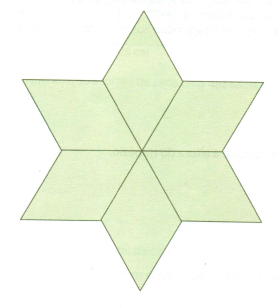
\includegraphics[width=0.7\linewidth]{8FMA28_imagens/pg147.png}\\\\\\\\\\\\\\\\
    			
    		\item Um terreno com o formato de um losango tem um ângulo de 120$^\circ$ e diagonal menor medindo 60 m. Qual é a área desse terreno?\\\\\\\\\\\\\\\\\\
    		\item Sabemos que a razão entre as medidas das diagonais de um losango é 1 : 3 e que o perímetro do losango é $12\sqrt{10}$ mm. Calcule a área desse losango em mm$^2$. \\\\\\\\\\\\\\\\
    		\item Um losango tem diagonais medindo 26 cm e 16 cm. A área do quadrilátero cujos vértices são os pontos médios dos lados do losango é:
    		\begin{enumerate}[a)]
    			\item 79 cm²
    			\item 81 cm²
    			\item 97 cm²
    			\item 104 cm²
    			\item 201 cm²\\\\\\\\\\\\\\\\
    		\end{enumerate}
    	    \item Unindo os pontos médios dos lados de um retângulo construímos um losango. Mostre que a área desse losango é a metade da área do retângulo.
	    \end{enumerate}
    $~$ \\ $~$ \\ $~$ \\ $~$
    \end{multicols}

\end{document}